\documentclass{beamer}

% for themes, etc.
\mode<presentation>{ 
\usetheme{Rochester} 
}

\usepackage{array}
\usepackage{graphicx}
\usepackage{tikz}
\usetikzlibrary{shapes, arrows, positioning}

\title[]{A Surrogate Approach Towards Validation and Uncertainty Quantification of Multiphysics Reactor Simulation Codes}
\subtitle[]{Thesis Prospectus}
\author[]{Artem Yankov}
\institute[]{University of Michigan}
\date{April 17, 2014}

% have this if you'd like a recurring outline
\AtBeginSection[]  % "Beamer, do the following at the start of every section"
{
\begin{frame}<beamer> 
\frametitle{Outline} % make a frame titled "Outline"
\tableofcontents[currentsection]  % show TOC and highlight current section
\end{frame}
}

\begin{document}

% this prints title, author etc. info from above
\begin{frame}
\titlepage
\end{frame}

% MOTIVATION
\section{Motivation}

%%%%%%%%%%%%%%%%%%%%%%%%%%%%%%%%%%%%%%%%%%%%%%%%%%%%%%%%%%%%%%%%%%%%%%%%%%%%%%%%%%%%%%%%
\begin{frame}
\frametitle{Background}

\begin{itemize}
  \item Physical phenomena is studied by conducting experiments. 
  \item Any data collected represents instances of underlying stochastic processes.  
  \item We build predictive computer models in an attempt to reproduce such observed physical phenomena.
  \item To accurately capture stochastic element of experiments, computer models should be probabilistic.  
  \item In other words, inputs to computer models have uncertainties associated with them that are propagated to any outputs of interest.
  \item Running computer simulations should be like conducting physical experiments. Computer experiments.      
\end{itemize}

\end{frame}
%%%%%%%%%%%%%%%%%%%%%%%%%%%%%%%%%%%%%%%%%%%%%%%%%%%%%%%%%%%%%%%%%%%%%%%%%%%%%%%%%%%%%%%%
\begin{frame}
\frametitle{Why Surrogates?}

\begin{itemize}
  \item We run computer simulations to meet design objectives under certain constraints. 
  \item Involves numerical optimization, calibration, and performing what-if analyses.
  \item Also, we're interested in determining which of our design variables have the greatest effects on simulation outcomes. 
  \item Thousands of simulations required to make this possible but...  
  \item Computer simulations that model real phenomenon like nuclear reactors often take $\mathcal{O}(\mbox{hours})$ or $\mathcal{O}(\mbox{days})$ to complete.
  \item Building a surrogate model for your expensive computer simulations can make everything listed above possible.   
\end{itemize}

\end{frame}
%%%%%%%%%%%%%%%%%%%%%%%%%%%%%%%%%%%%%%%%%%%%%%%%%%%%%%%%%%%%%%%%%%%%%%%%%%%%%%%%%%%%%%%%
\begin{frame}
\frametitle{What is a Surrogate Model?}

\begin{itemize}
  \item A model for the outcomes of (likely) expensive computer simulations that can be rapidly evaluated while simultaneously preserving the predictive capabilities of the original simulations.
  \item Want to intelligently choose subspace $\lbrace x_1, x_2, ..., x_N\rbrace \subset \mathbf{X}$ to sample expensive computer code to get $\lbrace y_1, y_2, ..., y_N\rbrace \subset \mathbf{Y}$.
  \item Learn fast mapping that approximates $\mathbf{X}\rightarrow\mathbf{Y}$.   
\end{itemize}

\begin{figure}
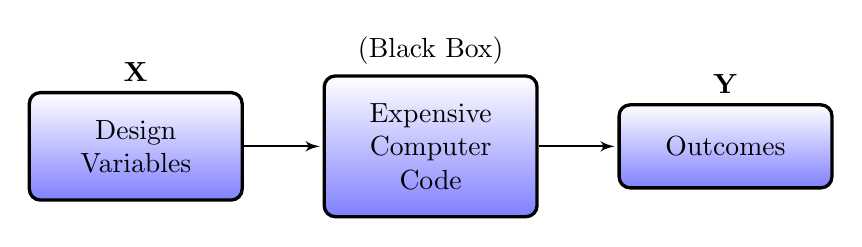
\begin{tikzpicture}[node distance=1cm, auto]  
\tikzset{
    mynode/.style={rectangle,rounded corners,draw=black, top color=white, bottom color=blue!50,very thick, inner sep=1em, minimum size=3em, text centered},
    myarrow/.style={->, >=latex', shorten >=1pt, thick},
    mylabel/.style={text width=7em, text centered} 
}  
\node[mynode, text width=2cm, label=$\mathbf{X}$] (design_vars) {Design Variables};  
\node[mynode, right= of design_vars, text width=2cm, label=(Black Box)] (computer_code) {Expensive Computer Code};
\node[mynode, right= of computer_code, text width=2cm, label=$\mathbf{Y}$] (outcomes) {Outcomes};
\draw[myarrow] (design_vars) edge node {} (computer_code);
\draw[myarrow] (computer_code) edge node {} (outcomes);
\end{tikzpicture}  
\end{figure}

\end{frame}

% PROPOSED APPLICATION
\subsection{Proposed Application}
%%%%%%%%%%%%%%%%%%%%%%%%%%%%%%%%%%%%%%%%%%%%%%%%%%%%%%%%%%%%%%%%%%%%%%%%%%%%%%%%%%%%%%%%
\begin{frame}
\frametitle{Proposed Application to Fuel Performance Modeling}

\begin{itemize}
  \item Fission Gas Release (FGR) refers to the phenomenon where Xenon and Krypton gases formed in UO$_2$ fuel rods are released into the rod filling gas.
  \item Causes pressure build-up and thermal conductivity degradation in the rod filling gas, potentially jeopardizing the safety of the reactor.
  \item Fission gas atoms generated in the fuel grains diffuse towards the grain boundaries. 
  \item Majority of the gas diffuses into grain-face gas bubbles, giving rise to grain-face swelling.
  \item Bubble growth brings about bubble coalescence and interconnection, eventually leading to the formation of a tunnel network through which the fission gas is released.       
\end{itemize}

\end{frame}   
%%%%%%%%%%%%%%%%%%%%%%%%%%%%%%%%%%%%%%%%%%%%%%%%%%%%%%%%%%%%%%%%%%%%%%%%%%%%%%%%%%%%%%%%
\begin{frame}
\frametitle{SIFGRS FGR Model}

\begin{itemize}
  \item Simple Integrated Fission Gas Release and Swelling (SIFGRS)
  \item Incorporates gas diffusion and precipitation in grains, growth and coalescence of gas bubbles at grain faces, thermal, athermal, steady-state, and transient gas release. 
  \item Through a direct description of the grain face gas bubble development, the fission gas swelling and release are calculated as coupled processes.
  \item Parameterized by, among others, linear heat rate, gas diffusion coefficient, surface tension of grain face bubbles, hydrostatic pressure, fuel grain radius, fuel porosity, and grain boundary sweeping. 
\end{itemize}

\end{frame}
%%%%%%%%%%%%%%%%%%%%%%%%%%%%%%%%%%%%%%%%%%%%%%%%%%%%%%%%%%%%%%%%%%%%%%%%%%%%%%%%%%%%%%%%
\begin{frame}
\frametitle{Ris\o~AN3 Experiment}

\begin{itemize}
  \item Validation case for fuel performance modeling in the Fumex-II database.
  \item Experiment consists of a base irradiation of four reactor cycles in the Biblis A pressurized water reactor.
  \item After the base irradiation period, a fuel rod is extracted and refabricated to a shorter length before undergoing a power ramp.
  \item Refabricated fuel rod is outfitted with various instrumentation such that fuel centerline temperature, FGR and rod internal pressure measurements can be obtained.    
\end{itemize}

\end{frame}
%%%%%%%%%%%%%%%%%%%%%%%%%%%%%%%%%%%%%%%%%%%%%%%%%%%%%%%%%%%%%%%%%%%%%%%%%%%%%%%%%%%%%%%%
\begin{frame}
\frametitle{Ris\o~AN3 Experiment Irradiation Profiles}

\begin{columns}
 \begin{column}{0.5\textwidth}
  \centering
  Base Irradiation History
  \includegraphics[width=1.\textwidth]{./base_irrad.png}
 \end{column}
 \begin{column}{0.5\textwidth}
  \centering
  Power Ramp Experiment
  \includegraphics[width=1.\textwidth]{./power_ramp.png}
 \end{column}
\end{columns}

\end{frame}
%%%%%%%%%%%%%%%%%%%%%%%%%%%%%%%%%%%%%%%%%%%%%%%%%%%%%%%%%%%%%%%%%%%%%%%%%%%%%%%%%%%%%%%%
\begin{frame}
\frametitle{Modeling Ris\o~AN3 Experiment with BISON}

\begin{itemize}
  \item BISON is a finite-element fuel performance modeling code that utilizes the SIFGRS model.
  \item SIFGRS parameters are quite generic and uncertain. 
\end{itemize}

\begin{columns}
 \begin{column}{0.5\textwidth}
  \centering
  Fission Gas Release
  \includegraphics[width=1.\textwidth]{./fgr_comparison.png}
 \end{column}
 \begin{column}{0.5\textwidth}
  \centering
  Fuel Centerline Temperature
  \includegraphics[width=1.\textwidth]{./tc_temp_comparison.png}
 \end{column}
\end{columns}

\end{frame}
%%%%%%%%%%%%%%%%%%%%%%%%%%%%%%%%%%%%%%%%%%%%%%%%%%%%%%%%%%%%%%%%%%%%%%%%%%%%%%%%%%%%%%%%
\begin{frame}
\frametitle{Modeling Ris\o~AN3 Experiment with BISON/MPACT}

\begin{itemize}
  \item No sense in comparing the output of a computer simulation to
experimental data unless the computer simulation is of high fidelity and capable
of reproducing the pertinent physics.
  \item MPACT is a neutronics code that provides detailed intrapin and azimuthally dependent
neutronics data in the fuel elements. 
  \item The two-way coupling scheme provided by BISON and MPACT provides the most accurate fuel performance modeling available for a nuclear reactor.
  \item Expensive! 
\end{itemize}

\end{frame}
%%%%%%%%%%%%%%%%%%%%%%%%%%%%%%%%%%%%%%%%%%%%%%%%%%%%%%%%%%%%%%%%%%%%%%%%%%%%%%%%%%%%%%%%
\begin{frame}
\frametitle{Modeling Ris\o~AN3 Experiment with BISON/MPACT}

\begin{itemize}
  \item BISON predictions of FGR and temperature fields stand to be improved by calibrating FGR parameters to experimental data.
  \item Calibration studies require $\mathcal{O}(10^3)$ function evaluations, which in this case are the coupled BISON/MPACT computer codes.
  \item Each simulation of the Ris\o~AN3 experiment will take a few hours.
  \item It's necessary to construct a surrogate for the calibration study!   
\end{itemize}

\end{frame}
%%%%%%%%%%%%%%%%%%%%%%%%%%%%%%%%%%%%%%%%%%%%%%%%%%%%%%%%%%%%%%%%%%%%%%%%%%%%%%%%%%%%%%%%

% SURROGATE CONSTRUCTION
\section{Surrogate Models}

% OVERVIEW
\subsection{Overview}
%%%%%%%%%%%%%%%%%%%%%%%%%%%%%%%%%%%%%%%%%%%%%%%%%%%%%%%%%%%%%%%%%%%%%%%%%%%%%%%%%%%%%%%%
\begin{frame}
\frametitle{Classic Overview}

\begin{figure}
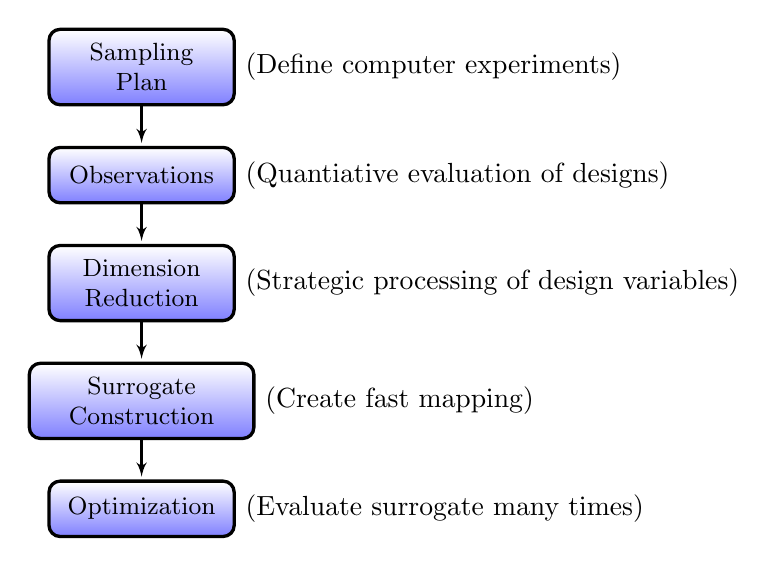
\begin{tikzpicture}[node distance=0.5cm, auto]  
\tikzset{
    mynode/.style={rectangle,rounded corners,draw=black, top color=white, bottom color=blue!50, very thick, inner sep=.5em, minimum size=2em, text centered, font=\small},
    myarrow/.style={->, >=latex', shorten >=1pt, thick}
}  
\node[mynode, text width=2cm, label=right:(Define computer experiments)](samp_plan) {Sampling Plan};
\node[mynode, below= of samp_plan, text width=2cm, label=right:(Quantiative evaluation of designs)](obs) {Observations};
\node[mynode, below= of obs, text width=2cm, label=right:(Strategic processing of design variables)](dim_red) {Dimension Reduction};
\node[mynode, below= of dim_red, text width=2.5cm, label=right:(Create fast mapping)](surr) {Surrogate Construction};
\node[mynode, below= of surr, text width=2cm, label=right:(Evaluate surrogate many times)](opt) {Optimization};
\draw[myarrow] (samp_plan) edge node {} (obs);
\draw[myarrow] (obs) edge node {} (dim_red);
\draw[myarrow] (dim_red) edge node {} (surr);
\draw[myarrow] (surr) edge node {} (opt);
\end{tikzpicture}  
\end{figure}

\end{frame}
%%%%%%%%%%%%%%%%%%%%%%%%%%%%%%%%%%%%%%%%%%%%%%%%%%%%%%%%%%%%%%%%%%%%%%%%%%%%%%%%%%%%%%%%
\begin{frame}
\frametitle{Kriging vs. anchored-ANOVA Collocation}

\begin{columns}
 \begin{column}{0.5\textwidth}
  Kriging
  \begin{itemize}
    \item Dimension reduction processed separately
    \item Sampling points random
    \item User determines how many points to use for sampling plan
    \item Interpolation by covariance basis functions
    \item More statistical approach
  \end{itemize}
 \end{column}
 \begin{column}{0.5\textwidth}
 anchored-ANOVA Collocation
  \begin{itemize}
    \item Dimension reduction inherent
    \item Sampling done on structured grid
    \item Sampling plan size dependent on number of design variables
    \item Polynomial interpolation
    \item More deterministic approach
  \end{itemize}
 \end{column}
\end{columns}

\end{frame}
%%%%%%%%%%%%%%%%%%%%%%%%%%%%%%%%%%%%%%%%%%%%%%%%%%%%%%%%%%%%%%%%%%%%%%%%%%%%%%%%%%%%%%%%
\subsection{Kriging}

\begin{frame}
\frametitle{Designing a Kriging Sampling Plan}

\begin{itemize}
  \item All surrogate models are built around a set of points at which the objective computer code is actually evaluated. 
  \item Intuitively, the surrogate accuracy is expected to decrease as one moves further away from such points. 
  \item Important to spread $N$ points as uniformly as possible across the design space.
  \item For Kriging, Latin Hypercube Sampling (LHS) is used to create a sampling plan.
  \item There is a notion of an optimized LHS sampling plan based on the maximin metric.   
\end{itemize}

\end{frame}
%%%%%%%%%%%%%%%%%%%%%%%%%%%%%%%%%%%%%%%%%%%%%%%%%%%%%%%%%%%%%%%%%%%%%%%%%%%%%%%%%%%%%%%%
\begin{frame}
\frametitle{Latin Hypercube Sampling}

\begin{itemize}
  \item Basis of LHS rests upon dividing the normalized space of each design variable into $n$ equally sized bins if $n$ samples are required. 
  \item As a result, when the $n$ samples are taken it is guaranteed that the entire
spectrum of each design variable's space has been visited.  
\end{itemize}
\centering
\includegraphics[width=0.58\textwidth]{./lhs.png}

\end{frame}
%%%%%%%%%%%%%%%%%%%%%%%%%%%%%%%%%%%%%%%%%%%%%%%%%%%%%%%%%%%%%%%%%%%%%%%%%%%%%%%%%%%%%%%%
\begin{frame}
\frametitle{Optimizing a LHS Plan}

\begin{itemize}
  \item The maximin metric describe by Morris and Mitchell makes use of two notions in an attempt to quantify the 'space-fillingness' of a sampling plan. 
  \item Unique distances between all points in the plan sorted in ascending order $\lbrace d_1, d_2, ..., d_m\rbrace$.
  \item Corresponding number of occurrences of each distance $\lbrace J_1, J_2, ..., J_m\rbrace$.  
  \item In words, the Morris and Mitchell criteria states that an optimized sampling plan will minimize all $J_i$ while maximizing the corresponding $d_i$. 
  \item The maximin sampling plan maximizes $d_1$, and among plans for which this is true, minimizes $J_1$, among plans for which this is true, maximizes $d_2$,....
\end{itemize}

\end{frame}
%%%%%%%%%%%%%%%%%%%%%%%%%%%%%%%%%%%%%%%%%%%%%%%%%%%%%%%%%%%%%%%%%%%%%%%%%%%%%%%%%%%%%%%%
\begin{frame}
\frametitle{Optimizing a LHS Plan}

\begin{itemize}
  \item The previous definition can be restated into a pseudo equivalent minimization problem.
\begin{equation}
\label{eq:Phi_q}
   \Phi_q(\textbf{X}) = \left(\sum_{j=1}^m J_j d_j^{-q} \right)^{1/q} \nonumber
\end{equation}
  \item The minimization of this equation and the Morris and Mitchell definition of the maximin sampling plan are used in unison to obtain a locally optimal sampling plan.
  \item Generate initial sampling plan, optimize for set of $q$ values using simulated annealing.  
  \item Resulting set of plans are contested directly against each other by explicit application of Morris and Mitchell's maximin definition. 
\end{itemize}

\end{frame}
%%%%%%%%%%%%%%%%%%%%%%%%%%%%%%%%%%%%%%%%%%%%%%%%%%%%%%%%%%%%%%%%%%%%%%%%%%%%%%%%%%%%%%%%
\begin{frame}
\frametitle{Kriging on a Sampling Plan}

\begin{itemize}
  \item Optimized sampling plan $\textbf{X}=\lbrace \textbf{x}^{(1)}, \textbf{x}^{(2)}, ... \textbf{x}^{(n)}\rbrace$. 
  \item At each datum $\textbf{x}^{(k)}$ a random process $Y(\textbf{x}^{(k)})$ induces an observation $y^{(k)}$.
  \item Resulting random field can be described with a mean value of $\textbf{1}\mu$ and a correlation matrix,
\begin{equation}
 \boldsymbol{\Psi} =
 \begin{pmatrix} 
	cor[Y(\textbf{x}^{(1)}), Y(\textbf{x}^{(1)})] & \cdots & 
		cor[Y(\textbf{x}^{(1)}), Y(\textbf{x}^{(n)})] \\
	\vdots & \ddots & \vdots \\ 
	cor[Y(\textbf{x}^{(n)}), Y(\textbf{x}^{(1)})] & \cdots & 
		cor[Y(\textbf{x}^{(n)}), Y(\textbf{x}^{(n)})]
 \end{pmatrix} \nonumber
\end{equation}  
\begin{equation}
   cor[Y(\textbf{x}^{(i)}), Y(\textbf{x}^{(l)})] = 
    \exp\left(-\sum_{j=1}^k \theta_j |x_j^{(i)} - x_j^{(l)} |^{p_j} \right) \nonumber
\end{equation}
\end{itemize}

\end{frame}
%%%%%%%%%%%%%%%%%%%%%%%%%%%%%%%%%%%%%%%%%%%%%%%%%%%%%%%%%%%%%%%%%%%%%%%%%%%%%%%%%%%%%%%%
\begin{frame}
\frametitle{Kriging on a Sampling Plan}

\begin{itemize}
  \item Given the formulation of the observations occurring at $\textbf{x}^{(k)}$ as instances of a stochastic process, the likelihood of seeing the observed data is,
\begin{eqnarray}
   L\left(\textbf{Y}^{(1)}, ..., \textbf{Y}^{(n)} | 
    \mu, \sigma, \lbrace \theta_1,..., \theta_k\rbrace, 
    \lbrace p_1,..., p_k\rbrace\right) = \nonumber \\
     \frac{1}{\left(2\pi\sigma^2\right)^{n/2}|\boldsymbol{\Psi}|^{1/2}}\times
     \exp\left[\frac{  \left(\textbf{y}-\textbf{1}\mu\right)^T
    \boldsymbol{\Psi}^{-1} \left(\textbf{y}-\textbf{1}\mu\right)}
    {2\sigma^2} \right] . \nonumber
\end{eqnarray} 
  \item Maximizing the log likelihood, 
   \begin{equation}
   	\hat{\mu} = \frac{ \textbf{1}^T\boldsymbol{\Psi}^{-1}\textbf{y} }
    		 	    {  \textbf{1}^T\boldsymbol{\Psi}^{-1}\textbf{1} } \nonumber
   \end{equation}
   \begin{equation}
   	\hat{\sigma}^2 = \frac{  \left(\textbf{y}-\textbf{1}\mu\right)^T
    			\boldsymbol{\Psi}^{-1} \left(\textbf{y}-\textbf{1}\mu\right)}{n}. \nonumber
   \end{equation}
\end{itemize}

\end{frame}
%%%%%%%%%%%%%%%%%%%%%%%%%%%%%%%%%%%%%%%%%%%%%%%%%%%%%%%%%%%%%%%%%%%%%%%%%%%%%%%%%%%%%%%%
\begin{frame}
\frametitle{Kriging on a Sampling Plan}

\begin{itemize}
  \item Substitute $\hat{\sigma}$ and $\hat{\mu}$ into log likelihood to get, concentrated ln-likelihood function.
   \begin{equation}
    \log(L) \approx -\frac{n}{2}\log\left(\hat{\sigma}^2\right) -
     \frac{1}{2} \log|\boldsymbol{\Psi}| \nonumber	
   \end{equation}
  \item Optimize with respect to the $\theta$ and $p$ parameters using global search algorithm.
  \item Once all optimizing parameters are available the goal is to utilize the parameters to build a model that makes function predictions on new points $\textbf{x}$.
\end{itemize}

\end{frame}
%%%%%%%%%%%%%%%%%%%%%%%%%%%%%%%%%%%%%%%%%%%%%%%%%%%%%%%%%%%%%%%%%%%%%%%%%%%%%%%%%%%%%%%%
\begin{frame}
\frametitle{Making Predictions with Kriging Surrogate}

\begin{itemize}
  \item Construct a vector of correlations with existing points and $\textbf{x}$,
   \begin{equation}
 	\boldsymbol{\psi} =
 	\begin{pmatrix} 
	 cor[Y(\textbf{x}^{(1)}), Y(\textbf{x})] \\
	 \vdots \\ 
	 cor[Y(\textbf{x}^{(n)}), Y(\textbf{x})] 
    \end{pmatrix}. \nonumber
   \end{equation} 
  \item  New predictions can be made at $\textbf{x}$ using the maximum likelihood estimator,
   \begin{equation}
    \hat{y}(\textbf{x}) = \hat{\mu} + 
   	 \boldsymbol{\psi}^T\boldsymbol{\Psi}^{-1}
   	  \left(\textbf{y} - \textbf{1}\hat{\mu}\right). \nonumber
   \end{equation}
  \item Prediction using kriging works to estimate a function value at a certain point by computing a weighted average of known function values in the vicinity of the objective points.
\end{itemize}

\end{frame}
%%%%%%%%%%%%%%%%%%%%%%%%%%%%%%%%%%%%%%%%%%%%%%%%%%%%%%%%%%%%%%%%%%%%%%%%%%%%%%%%%%%%%%%%
\subsection{Collocation and anchored-ANOVA}

\begin{frame}
\frametitle{Collocation and anchored-ANOVA Algorithmic Overview}

\begin{itemize}
  \item anchored-ANOVA: Decompose objective function into functions of one variable $f(x_i)$, two variables $f(x_i, x_j)$, three variables $f(x_i, x_j, x_k)$ as needed.
  \item Collocation: For each component in the decomposition construct a polynomial interpolant by sampling objective function at pre-defined points.
  \item The pre-defined points are determined by Smolyak Sparse Grids, and a selection of quadrature abscissas (e.g. Newton-Cotes). 
  \item Combine interpolants in decomposition to get an effective surrogate. 
\end{itemize}

\end{frame}
%%%%%%%%%%%%%%%%%%%%%%%%%%%%%%%%%%%%%%%%%%%%%%%%%%%%%%%%%%%%%%%%%%%%%%%%%%%%%%%%%%%%%%%%
\begin{frame}
\frametitle{Numerical Interpolation in 1D}

\begin{itemize}
  \item First, pick a set of $m_i$ collocation points.   
  \item Evaluate objective function at all collocation points.
  \item Interpolated function is a linear expansion of some basis $a_j^i$ (e.g. Lagrange polynomials) with weights $f\left(x_j^i\right)$.  
\end{itemize}

\begin{equation} 
    U^i = \sum_{j=1}^{m_i} 
     f\left(x_j^i\right) a_j^i \nonumber
\end{equation}

\end{frame}
%%%%%%%%%%%%%%%%%%%%%%%%%%%%%%%%%%%%%%%%%%%%%%%%%%%%%%%%%%%%%%%%%%%%%%%%%%%%%%%%%%%%%%%%
\begin{frame}
\frametitle{Clenshaw-Curtis Collocation Points}

\begin{itemize}  
  \item Clenshaw-Curtis points consist of the extrema of Chebyshev polynomials. 
  \item $n + 1 $ abscissas can exactly integrate polynomials of degree $n$.
  \item Points have the advantage of being nested.
\end{itemize}
\begin{equation}
    x_{j}^{i} = \left\{
     \begin{array}{cr}
       \cos\frac{\pi(j-1)}{m_i-1}   & j=1,...,m_i \text{ if } i>1 \\
       0   &  j=1 \text{ if } i=1
     \end{array}
   \right. \nonumber
\end{equation} 
\begin{equation} 
    m_i = \left\{
     \begin{array}{cr}
      2^{i-1}+1   & i>1 \\
      1   & i=1
     \end{array}
    \right. \nonumber
\end{equation}

\end{frame}
%%%%%%%%%%%%%%%%%%%%%%%%%%%%%%%%%%%%%%%%%%%%%%%%%%%%%%%%%%%%%%%%%%%%%%%%%%%%%%%%%%%%%%%%
\begin{frame}
\frametitle{Basis Functions}

\begin{itemize}  
  \item Lagrange characteristic polynomials are plagued by the fact that each evaluation requires $\mathcal{O}(m_i^2)$ operations and often the computation is numerically unstable.
  \item Instead the barycentric form of Lagrange characteristic polynomials is used to form a basis. 
\begin{equation} 
    a_j^i = \left\{
     \begin{array}{cc}
      1   & \text{ if } i=1 \\
      \displaystyle \frac{\frac{w_j^i}{x-x_j^i} }
       {\sum_{j=0}^{m_i} 
        \frac{w_j^i}{x-x_j^i}}   & j=1,...,m_i \text{ for } i>1
     \end{array}
    \right. \nonumber
\end{equation}
  \item For Clenshaw-Curtis collocation points the barycentric weights are given by,
\begin{equation} 
    w_j^i = (-1)^{j+1}\delta_j^i \hspace{1 cm}
     \delta_j^i = \left\{
                   \begin{array}{cc}
                    .5   & j=1 \text{ or } j=m_i \\
                    1   & \text{ else }  
				   \end{array}
				  \right. . \nonumber                   
\end{equation}        
\end{itemize}

\end{frame}
%%%%%%%%%%%%%%%%%%%%%%%%%%%%%%%%%%%%%%%%%%%%%%%%%%%%%%%%%%%%%%%%%%%%%%%%%%%%%%%%%%%%%%%%





% APPLICATION OF SURROGATE METHODS
\section{Application of Surrogate Models}

% EXTRAS
\section{Extras}

%%%%%%%%%%%%%%%%%%%%%%%%%%%%%%%%%%%%%%%%%%%%%%%%%%%%%%%%%%%%%%%%%%%%%%%%%%%%%%%%%%%%%%%%
\begin{frame}
\frametitle{Sparse Grid Mechanics Example}

\begin{itemize}
  \item Consider a function of two dimensions $f(x_1, x_2)$ ($d=2$). 
  \item Let's calculate the Level 1 (q=3) Smolyak sparse grid interpolant for $f$, A(q=3, d=2).
\end{itemize}

\begin{equation}
\begin{array}{c}
 A(3,2) = A(2,2) + \Delta A(3,2) \\
 = \Delta A(2,2) + \Delta A(3,2)
\end{array} \nonumber
\end{equation}

\end{frame}


\end{document}